\section{Pedestrian Detection} \label{pedestrian}

\begin{figure}[!htbp]
    \centering
    \centerline{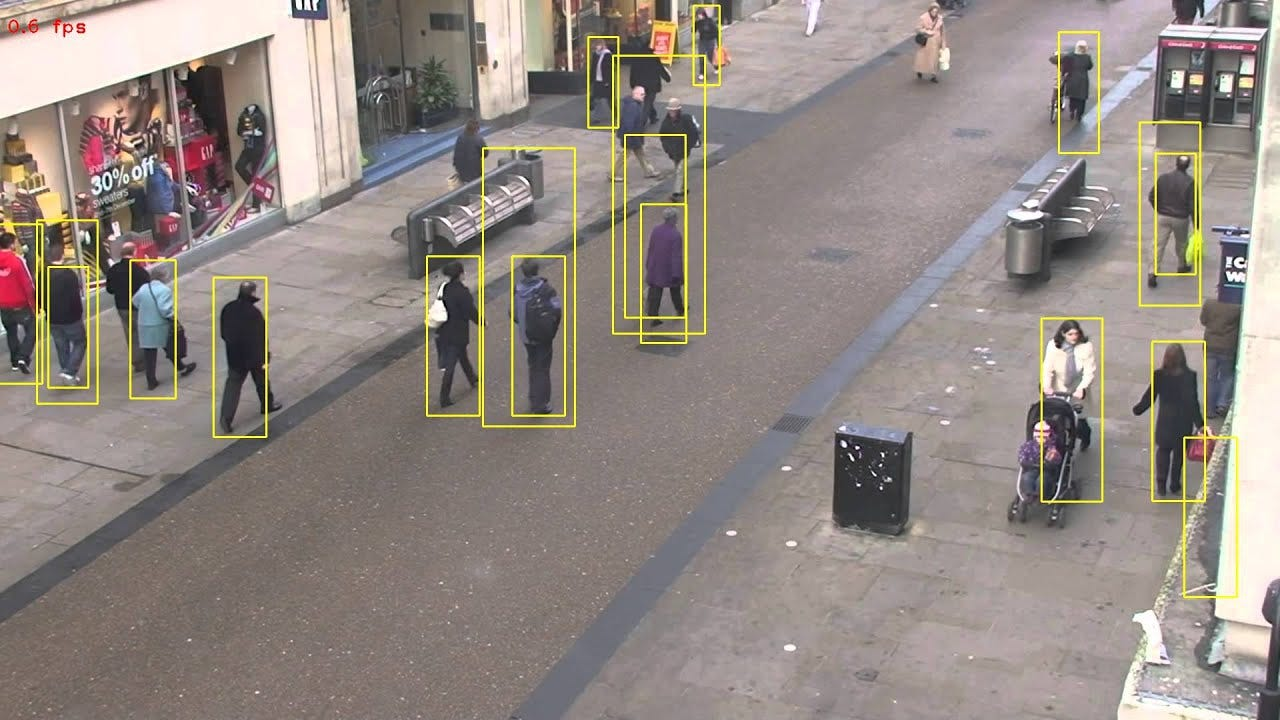
\includegraphics[width=0.8\linewidth]
    {images/pedestrian_detection.jpg}}
    \caption{Example of pedestrian detection \cite{agarwalPedestrianDetectionCount2021}}
    \label{fig:pedestrian_ex}
\end{figure}

Numerous studies have grappled with the multifaceted challenges of pedestrian detection, providing valuable insights to advance this field. One work tackled the issue of deteriorating model performance in the face of changing environmental lighting conditions \cite{kruthiventiLowlightPedestrianDetection2017}, while another introduced an algorithm that leveraged scale and occlusion visual cues, outperforming existing methods in pedestrian detection \cite{wangPedestrianDetectionCrowded2016}.

Efficiency became the focus of a study that devised a streamlined model based on a modified ShuffleNet and YOLOv3, resulting in a real-time detection system \cite{xuEfficientPedestrianDetection2022}. Other works made use of infrared imagery to improve pedestrian detection in nocturnal conditions \cite{parkRobustThermalInfrared2022, liInfraredImagePedestrian2021}, and several studies explored the advantages of multi-scale feature fusion to enhance the overall performance of pedestrian detection models \cite{chenMultiscaleFeatureFusion2023, huangPedestrianDetectionBased2022, fuPedestrianDetectionMethod2022, mengMPDFFMultisourcePedestrian2022}.

Another avenue for enhancing pedestrian detection involves the incorporation of attention mechanisms into existing models. Incorporating channel attention into a specific algorithm, for instance, led to a lower MR$^{-2}$ compared to the original method \cite{liPedestrianDetectionAlgorithm2021}. Particularly, the Convolutional Block Attention Module (CBAM) has gained attention for its capacity to enhance various metrics, including accuracy \cite{fengPedestrianDetectionBased2020, fanImprovedYOLOv5Algorithm2022, chenMultiscaleFeatureFusion2023}.


% The emergence of the COVID-19 pandemic introduced a new research and application domain: the utilization of pedestrian detection in monitoring public health.

% With concerns for personal health, the well-being of others, and the safety of the environment during the pandemic \cite{srinivasanCOVID19MonitoringSystem2021, rakhsithFaceMaskSocial2021}, research efforts have focused on developing models that can assist in enforcing public health protocols, such as social distancing and mask-wearing. Promising results have been obtained through studies utilizing YOLOv3 for social distancing detection and MobileNetV2 for face mask detection \cite{srinivasanCOVID19MonitoringSystem2021, rakhsithFaceMaskSocial2021}. Furthermore, YOLOv4 has been employed successfully to handle both tasks, yielding similarly positive outcomes \cite{bhambaniRealtimeFaceMask2020, lathasoniyaRealTimeSafe2022}.


